\section{Przegląd środowisk uruchomieniowych}\label{env}
Do czasów powstania pierwszego środowiska uruchomieniowego JavaScript, możliwość uruchomienia programów ograniczał się do przeglądarki. Przeglądarki nie pozwalały na dostęp do pików, co nie pozwalało zapisywać dodatkowych plików na maszynie klienta. W ten sposób powstało pierwsze środowisko uruchomieniowe JavaScript w 2009, czyli \textit{NodeJS}.

Środowiska uruchomieniowe pozwalają na uruchomienie skryptów JavaScriptu poza przeglądarką. Pozwoliło to językowi JavaScript stać się językiem generalnego użycia, co dla programistów stworzyło możliwość tworzenia aplikacji desktopowych, pozwoliło także na tworzenie API. Atutem środowiska powstałego w 2009 roku był asynchroniczny dostęp do systemu plików, pozwoliło to na optymalizacje operacji wejścia/wyjścia dla dużych skalowalnych aplikacji webowych.

Po upływie czasu zauważono, że NodeJS nie jest na tyle szybkim językiem do tworzenia serwerów, które mogły przekazywać informacje poprzez żądania HTTP. Stworzono także menadżera paczek, który pozwalał z jednego repozytorium pobierać paczkę, która umożliwiała uzupełnić braki samego środowiska. W czasie rosnącej popularności także zauważono, że rośnie liczba bibliotek, które korzystały ze słabych punkty samego środowiska, dzięki którym pozyskano wrażliwe dane.

W odpowiedzi na narastające problemy w związku wolnym działaniem środowiska NodeJS, zaczęto prace nad nowym bezpieczniejszym oraz wydajniejszym środowiskiem uruchomieniowym. W ten sposób powstało środowisko \textit{Deno}, które stworzył w oparciu o silnik JavaScript V8 twórca NodeJS. Początkowo zostało zbudowane w oparciu o język Go, który został zamieniony na język Rust. Twórcy Deno chcieli, aby paczki były dostępne pod linkiem, co oznacza szybsze przejście do samych pakietów oraz ich dokumentacji. Dodatkowo Deno wprowadziło natywne wsparcie do TypeScript'a, pozwoliło to na statyczne typowanie samych bibliotek oraz zewnętrznych pakietów. Wersja 1.0 Deno, została wydana 13 maja 2020 roku.

Środowiska zostały wybrane na podstawie corocznej ankiety \textit{State of JS} \cite{State_of_js:2022}, w której programiści wybierają narzędzia, które są przez nich najczęściej używane. Na liście z 2022 roku, można zauważyć, że nie zostało wymienione środowisko \textit{Bun}, spowodowane jest to wydaniem wersji 1.0 we wrześniu 2023 roku. Możemy jednakże zauważyć, że Bun pojawia się w pracach \cite{NodeAndBun}, które analizują wydajność NodeJS oraz Bun.

Bun jako najmłodszy reprezentant środowisk wyróżnia się swoją szybkością, wbudowanym w sam silnik menadżer pakietów i bundler, co ułatwiło deweloperom kompresowanie samych aplikacji webowych. Środowisko to zostało napisane w języku Zig, dzięki czemu zawdzięcza swoją szybkość.

W tym rozdziale znajduje się opis wybranych do badań środowisk uruchomieniowych JavaScript.

\subsection{NodeJS}
NodeJs jest to powstałe w 2009 środowisko uruchomieniowe, które pozwoliło na znaczne rozwinięcie samego środowiska języka JavaScript o dodatkowe funkcjonalności. Środowisko zostało oparte o silnik V8 od Google, które pozwoliło na uruchamianie kodu poza przeglądarką, które było do powstania środowiska niemożliwe. Wprowadziło to także możliwość tworzenia dynamicznych stron, co spowodowało rozwój bibliotek związanych z tworzeniem widoków. Aktualnie środowisko jest rozwijane przez OpenJs Fundation, sama organizacja wprowadza zmiany do samego środowiska np. obsługa zmiennych środowiskowych pobieranych z pliku.

Środowisko zostało zbudowane o paradygmat zdarzeniowy, stosuje się w nim pętle zdarzeniową, która nasłuchuje konkretnych zdarzeń, a następnie zdarzenia, które są umieszczone w stosie zdarzeń są wykonywane w kolejności FIFO. \cite{event_loop} Omówioną architekturę przedstawiono na Rysunku \ref{fig:eventLoop}.

\begin{figure}[h]
  \centering
  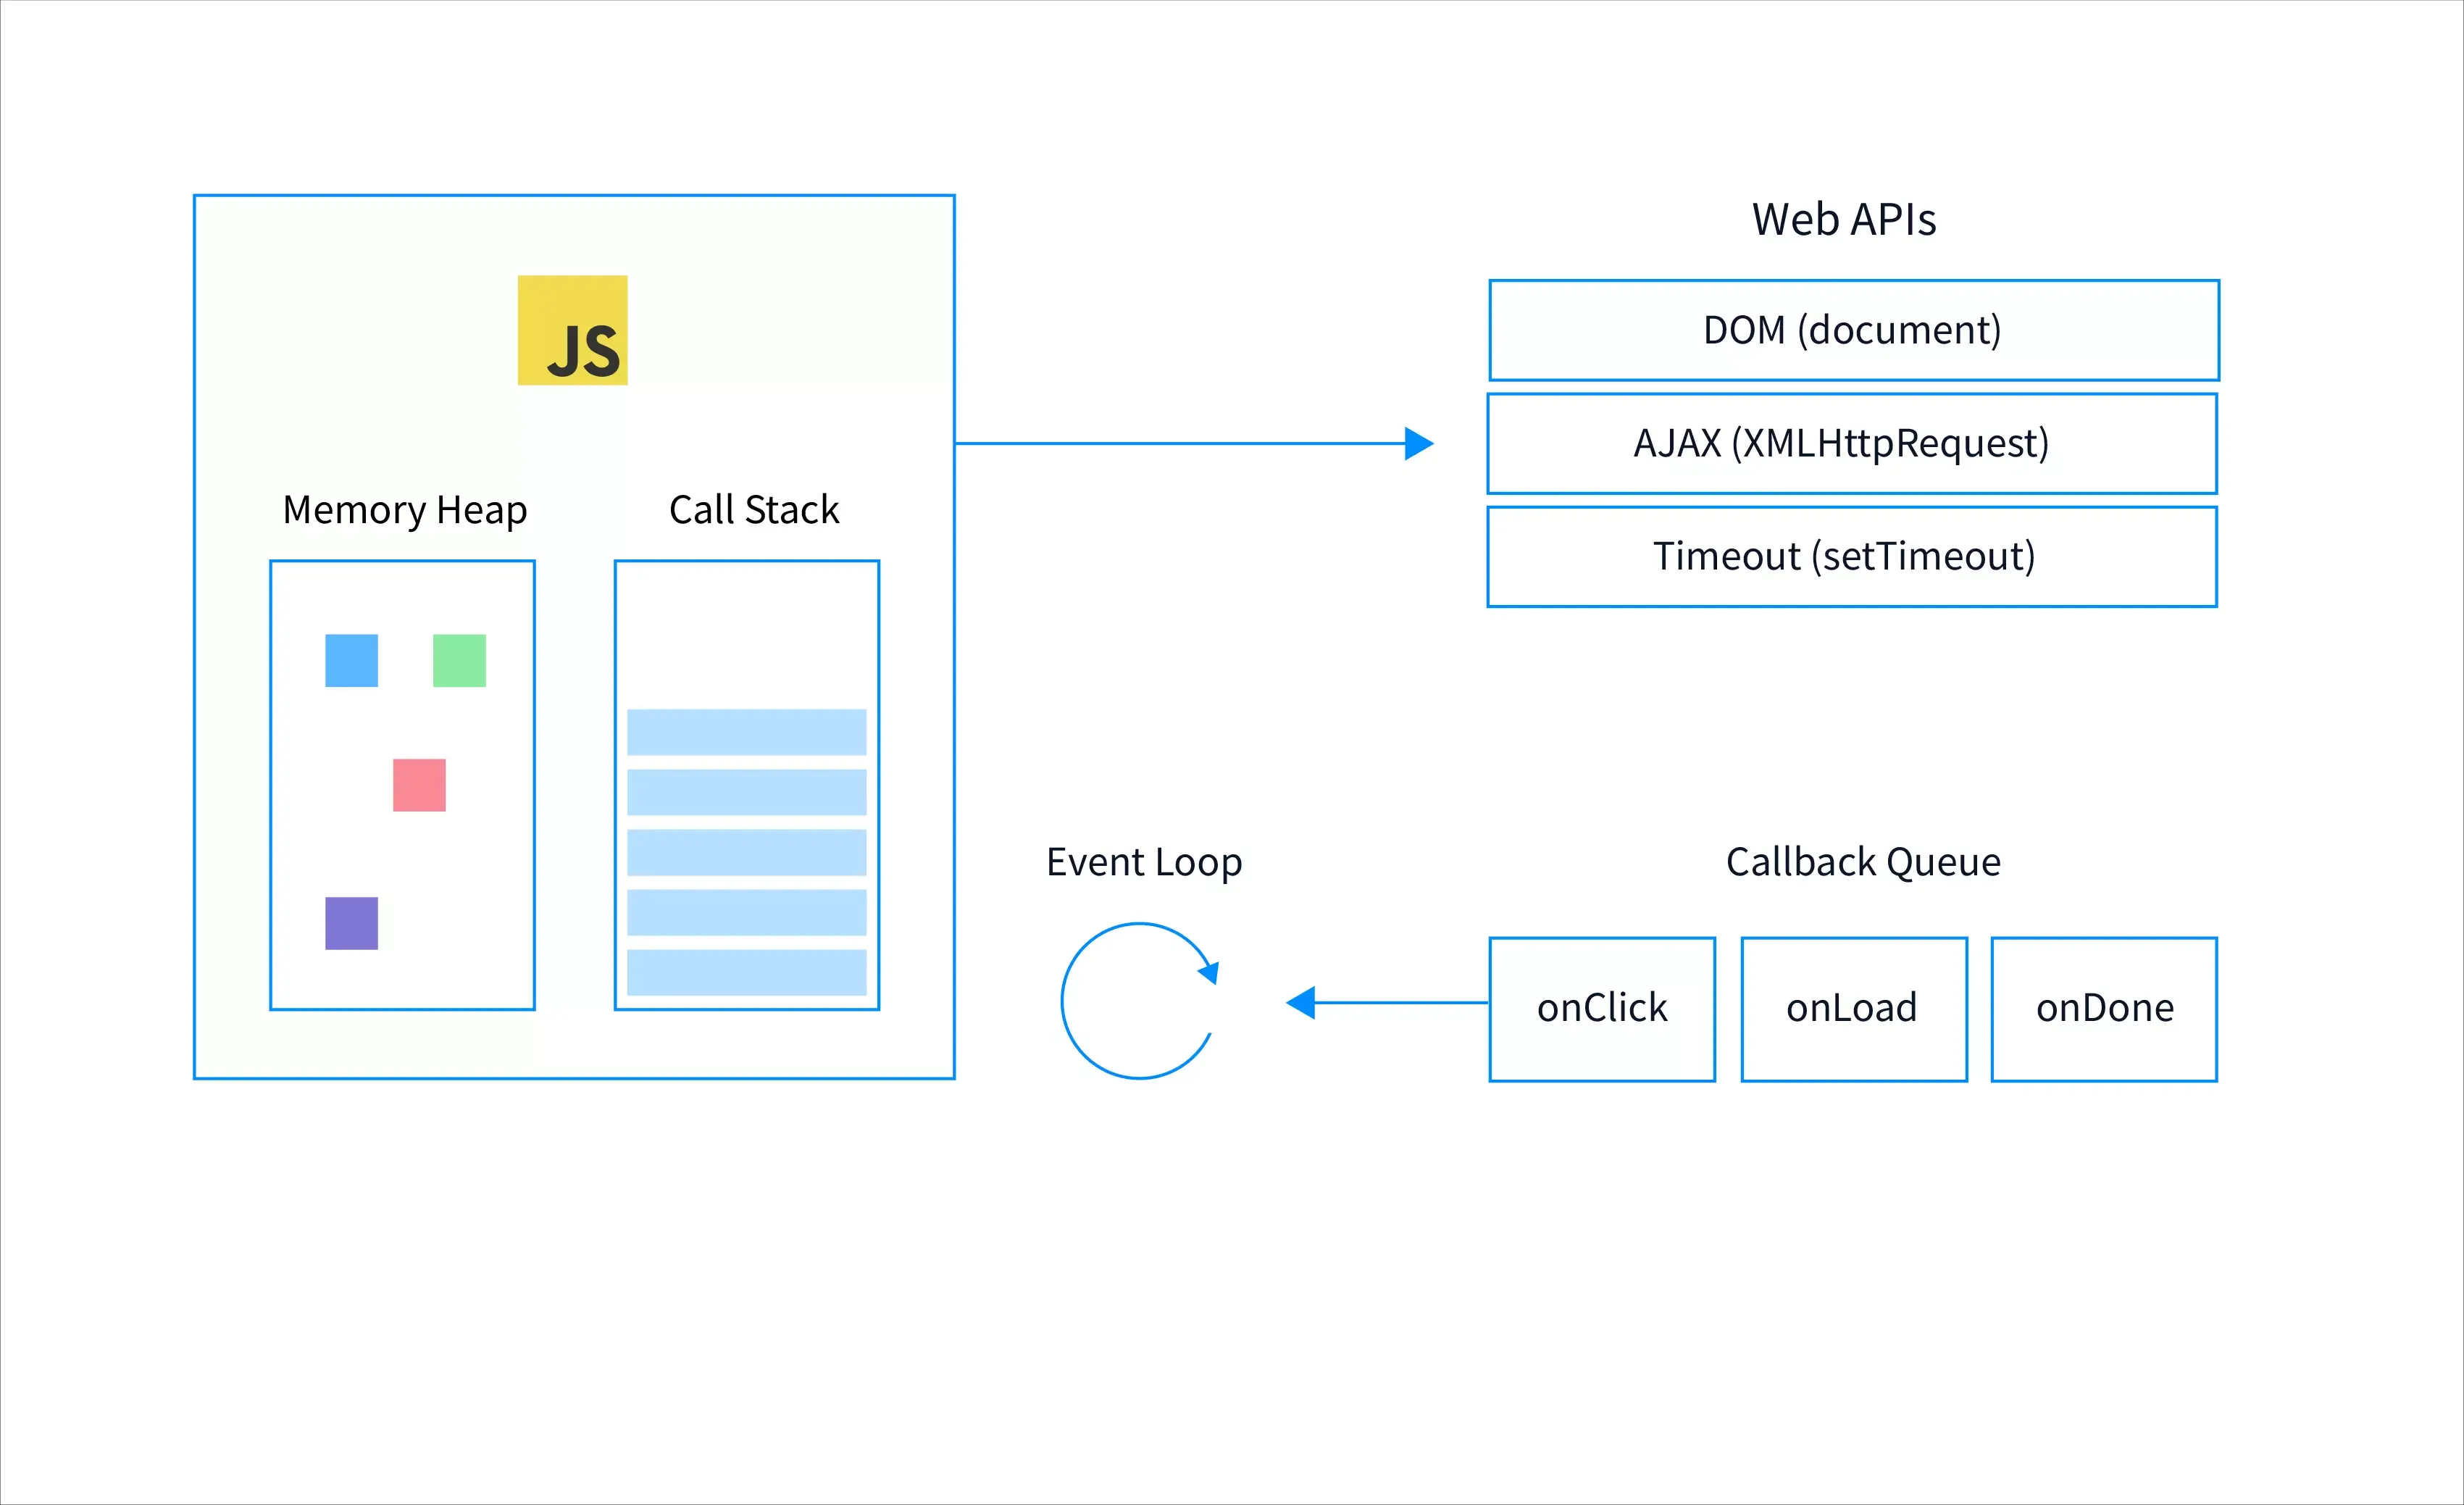
\includegraphics[width=0.9\textwidth]{Figures/eventLoop.png}
  \caption{Architektura zdarzeń dla NodeJS Źródło: \cite{event_loop}}
  \label{fig:eventLoop}
\end{figure}

Zastosowanie powyższej architektury pozwoliło na wprowadzenie asynchronicznej obsługi operacji wyjścia wyjścia. Dzięki tej architekturze, NodeJs jest środowiskiem, w którym produkuje się skalowalne aplikacje internetowe. Środowisko to zostało rozwijane, gdzie dodatkowo wprowadzono moduły odpowiedzialne za funkcje kryptograficzne, funkcje odpowiedzialne za sieci oraz obsługę binarnych danych.

Środowisko posiada własny menadżer paczek nazywający się \textit{npm}. Menadżer \textit{npm} został zaprezentowany w 2010 roku \cite{npm}, rok od powstania samego środowiska. Korzystając z menadżer, deweloperzy mogą udostępniać biblioteki zrobione specjalnie pod NodeJs. Obecnie jest zarejestrowane 2.1 miliona bibliotek \cite{npm}, które znajdują się na w \textit{npm}. Na przestrzeni czasu, można zauważyć, że \textit{npm} nie jest wydajnym menadżerem, dlatego też powstały alternatywy takie jak: \textit{yarn} \cite{yarn} oraz \textit{pnpm} \cite{pnpm}. 

W środowisku można pisać w kilku językach programowania, niestety nie odbywa się to bez dodatkowej konfiguracji projektu. Sam NodeJs odczytuje tylko i wyłącznie programy transpilowane lub napisane w JavaScript. Na dzień dzisiejszy środowisko wspiera transpilowanie z kilku języków takich jak: CoffeeScript, Dart, TypeScript oraz ClojureScript.

\subsection{Deno}
Deno jest to środowisko uruchomieniowe, które zostało podobnie jak NodeJs zbudowane na podstawie silnika V8 od Google. Współautorem środowiska jest Ryan Dahl, który jest współtwórcą Deno. Środowisko spełnia także rolę menadżera paczek, który pozwala na pobieranie paczek z wykorzystaniem linków. W przeciwieństwie do NodeJS, które nie posiada tak szybkiego sposobu na wykorzystanie zewnętrznych bibliotek.

Bazowanie na silniku V8 oraz przepisaniu części funkcjonalności z wykorzystaniem języka Rust, pozwoliło na zwiększenie wydajności samego silnika. Wydajność samego Deno została zbadana w pracy \cite{deno_performance}, w której porównano wydajność samego środowiska z NodeJs. W pracy wykazano, że Deno jest szybsze od NodeJs, co pozwala na zwiększenie wydajności samego środowiska. W tej pracy sprawdzono wydajność wysyłanych żądań HTTP, w której wykazano, że Deno jest szybsze od NodeJs. Rysunek \ref{fig:deno_vs_node} przedstawia wyniki porównania wydajności Deno oraz NodeJs.

\begin{figure}[H]
  \centering
  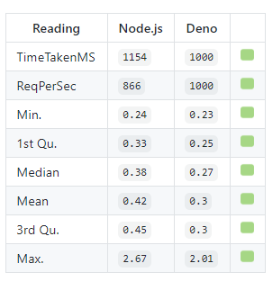
\includegraphics[width=0.52\textwidth]{Figures/deno_performance.png}
  \caption{Wyniki testu wydajnościowego Deno oraz NodeJs Źródło: \cite{deno_performance}}
  \label{fig:deno_vs_node}
\end{figure}

Deno jako środowisko jest bezpieczniejsze od NodeJs, ze względu na ograniczenie dostępu do plików, skutkuje to zwiększeniem bezpieczeństwa samego środowiska. W NodeJs, dostęp do plików jest nieograniczony, co pozwala na dostęp do wszystkich plików na maszynie. Należy także wspomnieć, iż Deno także nie zezwala na ruch sieciowy bez wskazania właściwej flagi. W ten sposób stworzono środowisko, które zostało zabezpieczone przed atakami z zewnątrz.

Deno jako środowisko posiada wbudowane wsparcie dla TypeScript, pozwala to na statyczne typowanie samych bibliotek oraz zewnętrznych pakietów. W przeciwieństwie do NodeJs, gdzie wymagane jest aby zainstalować dodatkowe pakiety, które pozwolą na statyczne typowanie. W Deno, nie musimy instalować dodatkowych pakietów, zwiększa to produktywność programistów oraz zmniejsza możliwość wystąpienia błędu.

Deno jako środowisko posiada wbudowany bundler, umożliwia to kompresowanie aplikacji do małej liczby plików. W NodeJs, musimy zainstalować dodatkowe pakiety, które pozwolą na kompresowanie samej aplikacji. Same pakiety powoduje znaczne zwiększenie rozmiaru aplikacji.

Samo środowisko udostępnia także wbudowane narzędzia pozwalające na tworzenie aplikacji webowych w oparciu o składnie JSX bądź TSX. Dzięki czemu środowisko jest rozszerzone, deweloperzy nie muszą tworzyć repozytoriów odpowiedzialnych tylko za widoki przedstawione na stronie. Pozwala to na tworzenie jednej wspólnej bazy kodowej, co pozwala na szybszy rozwój aplikacji.

Misją samego środowisko jest ujednolicanie bazy kodowej napisanych w tym środowisku. Z tego powodu Deno posiada swój własny \textit{formater} kodu, umożliwiający usunięcie pakietów tj. prettier z bazy kodowej danego projektu. 

\subsection{Bun}
Bun \cite{bun} jest to najmłodsze środowisko uruchomieniowe, stworzone przez Jarreda Summera. Wersja 1.0 została zaprezentowana we wrześniu 2023 roku. Środowisko to zostało zbudowane na podstawie silnika JavaScript WebKit, jest to rozwiązanie od firmy Apple wykorzystywane w przeglądarce Safari.

Sam autor środowiska twierdzi, że środowisko jest szybsze od NodeJs oraz Deno, co pozwala na zwiększenie wydajności samego środowiska. W pracy \cite{NodeAndBun} porównano wydajność samego środowiska z NodeJs oraz Bun. W pracy wykazano, że Bun jest szybsze od NodeJs, gdzie sprawdzono wydajność środowiska w kontekście aplikacji webowych. Praca wykorzystuje tylko metrykę liczby żądań na sekundę, nie przedstawia wykorzystanej pamięci. Rysunek \ref{fig:bun_vs_node} przedstawia wyniki porównania liczby żądań HTTP przy założonej liczby współbieżnych połączeń z serwerem połaczeniach Bun oraz NodeJs.

\begin{figure}[H]
  \centering
  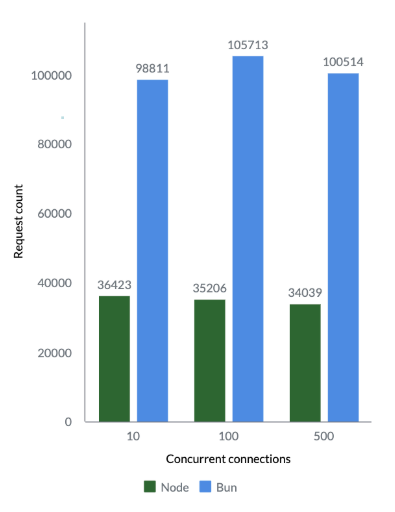
\includegraphics[width=0.47\textwidth]{Figures/bun_bench_node.png}
  \caption{Wyniki testu wydajnościowego Bun oraz NodeJs Źródło:\cite{bun_test}}
  \label{fig:bun_vs_node}
\end{figure}

Sam twórca opracował testy wydajnościowe, sprawdzające wydajność środowiska, ich rezultaty są opublikowane na stronie \cite{bun_test}. Autor korzystał z wbudowanych w silniki metod, które odpowiadają za SSR (\textit{ang. Server Side Rendering}), co imituje środowisko przeglądarki. Jednakże możemy zauważyć, że jest to prosta strona, która zawiera tylko tekst. W testach wydajnościowych sprawdzono wydajność samego środowiska, w których wykazano, że Bun jest szybsze od NodeJs. Rysunek \ref{fig:bun_bench} przedstawia wyniki porównania liczby żądań HTTP na sekundę.

\begin{figure}[H]
  \centering
  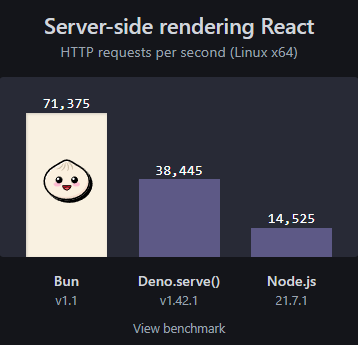
\includegraphics[width=0.47\textwidth]{Figures/bun_bench.png}
  \caption{Wyniki testu wydajnościowego Bun oraz NodeJs Źródło: \cite{bun_test}}
  \label{fig:bun_bench}
\end{figure}

To co wyróżnia środowisko od pozostałych to wbudowany menadżer pakietów, który pozwala na integracje z \textit{npm} \cite{npm} oraz pozwala na importowanie paczek z samego NodeJs. Pozwala to na integracje z powstałymi już projektami w NodeJs. Samo środowisko też nie potrzebuje pliku \textit{package.json} \cite{package_structure}, które w NodeJs jest wymagane. Samo środowisko tworzy jeden plik odpowiedzialny za wszystkie zależności wykorzystywane w projekcie.

Sprawdzenie jakości kodu jest ułatwione, dla użytkowników środowiska ze względu na wbudowane środowisko testowe. Pozwala to na zrezygnowanie z dodatkowych bibliotek odpowiedzialnych za tworzenie testów. Samo środowisko posiada asercję oraz dodatkowe funkcje, które pozwalają na tworzenie testów jednostkowych. Niektóre funkcje pozwalają na niewykonywanie testów w zależności od warunków dla na przykład wyłączenie danego testu w zależności od architektury danego systemu. W dokumentacji znajduje się przykład samej asercji, który przedstawiono na Listingu \ref{lst:bun_assert}.

\begin{centering}
  \begin{lstlisting}[caption={Przykład asercji w środowisku Bun},label={lst:bun_assert},captionpos=b]
    const macOS = process.arch === "darwin";
    test.skipIf(macOS)("runs on non-macOS", () => {
      // runs if *not* macOS
    });
  \end{lstlisting}
\end{centering}
